\section{Experimental evaluation}\label{sec:exp-evaluation}
We evaluated the above mentioned greedy heuristics-based approach in Apache Spark. Spark's SQL optimizer allows passing the optimizer rules externally to the application. We implemented an optimizer that takes the optimized plan as input and based on the heuristics proposed, reorders the joins wherever applicable. It is assumed that the table sizes are available in the Spark optimized plan before applying this rule. We used the TPC DS~\cite{b14}  dataset (scale 100) non-partitioned dataset for evaluating the performance. The experiments were run on a 5 node Apache Spark cluster on AWS with machine type r4.4xlarge.

Out of 100 TPC-DS~\cite{b14}  queries, at least one join in the 38 queries was reordered. We saw on average  For the queries not reordered, the performance would be the same as before. Figure \ref{performance_number} compares shows the improvement in percentages for the queries observed. Queries where difference were very low have been removed.

\begin{figure}[ht]
    \centerline{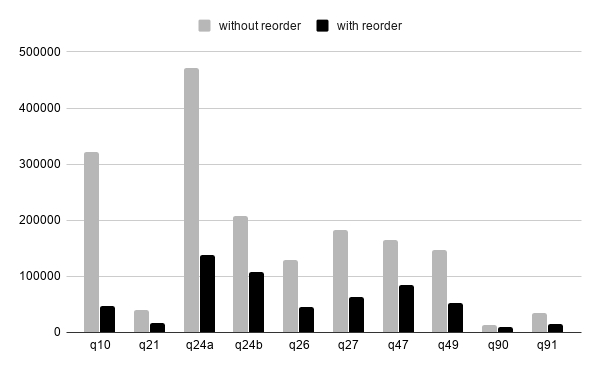
\includegraphics[width=7cm]{fig/chart.png}}
    \caption{Performance comparison of reordered queries}
    \label{performance_number}
\end{figure}

Out of all reordered queries, 5.1\% queries showed more than 20\% improvement, 15.4\% queries showed between 10 to 20\% improvement, 51.3\% queries showed between 0 to 10\% improvements and degraded 7.7\% queries showed the degradation of less than 5-10\%.
There were around 20\% we saw degradation of less than 5\% which on cloud environment can happen due to multiple reasons like noisy neighbor problem, object store latency fluctuations etc so can be ignored.

\begin{figure}[ht]
\centerline{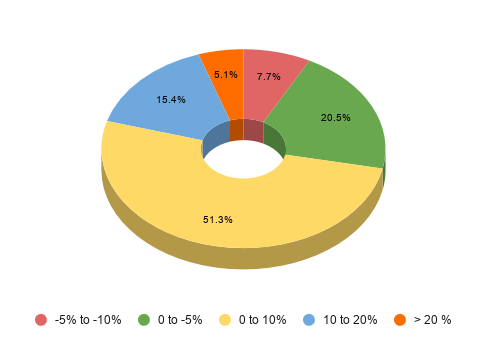
\includegraphics[width=7cm]{fig/pie.png}}
\caption{Performance distribution of reordered queries}
\label{performance_pie_chart}
\end{figure}

Let's consider query 21 of TPC-DS benchmark. An oversimplified query plan for the query is depicted in Figure \ref{without-reorder}. The join order in the plan is same as one given in the query. \texttt{inventory} table first joins with the \texttt{warehouse} table. The result is then joined with \texttt{item} and \texttt{date\_dim} tables respectively

\begin{figure}[ht]
\centerline{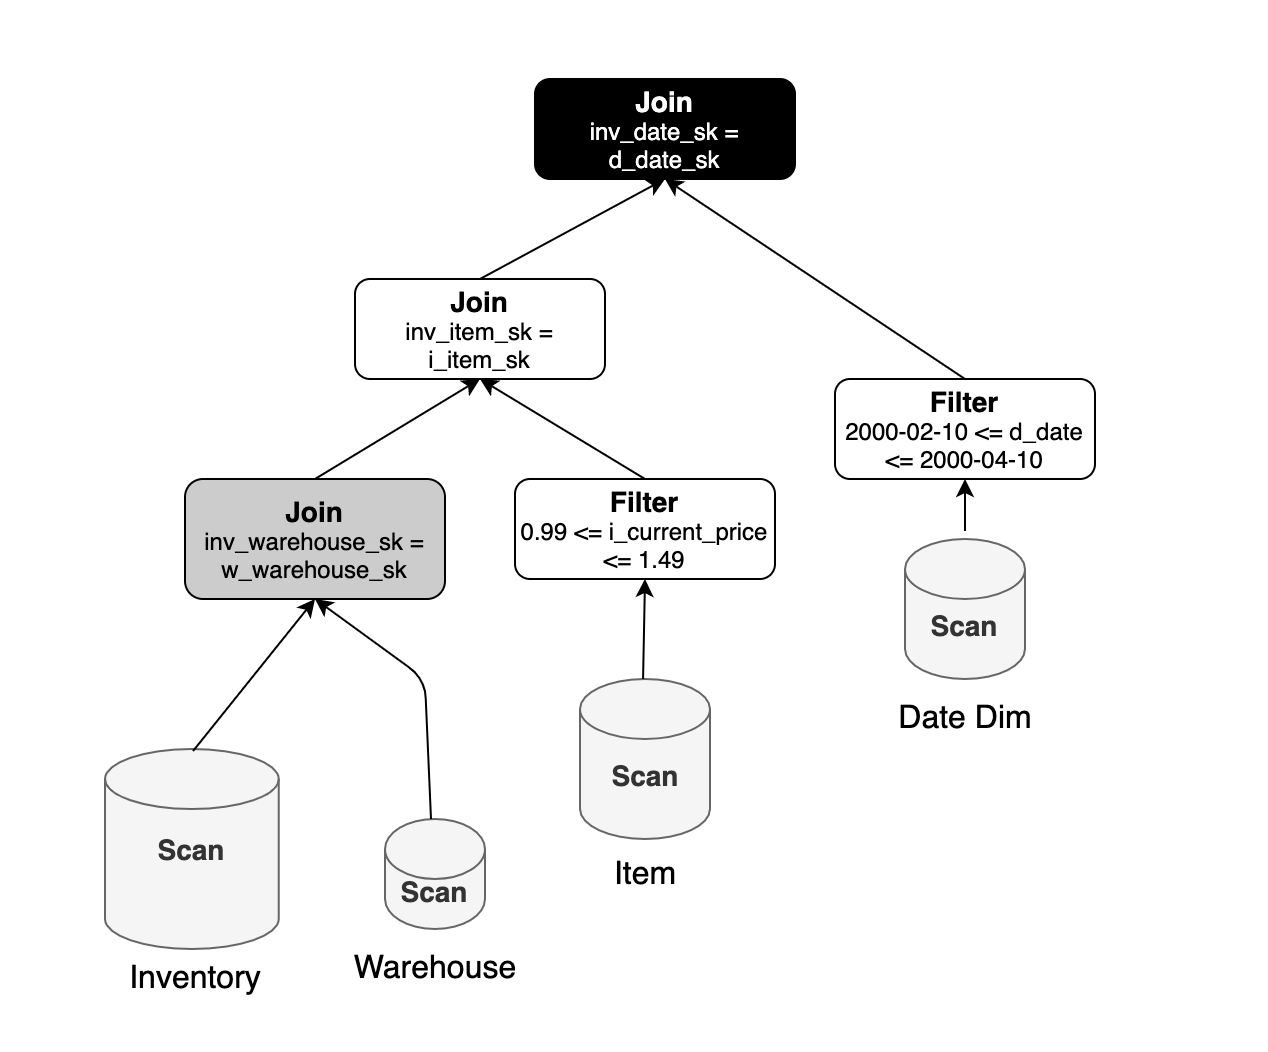
\includegraphics[width=7cm]{fig/without-reorder.png}}
\caption{Query 21 user order}
\label{without-reorder}
\end{figure}

Initially, we extract all consecutive joins from the query plan such that there is only a Project between the two Joins. Once we have the plans of left and right sub-tree and join conditions for each join, we try to extract the dominant Fact table and the dimensions tables. Table \texttt{inventory} is part of the of all three join conditions. So it becomes a candidate for being the fact table and all other tables as dimensions table. In dimensions tables, \texttt{inventory} table has the largest size followed by \texttt{item}, \texttt{date\_dim} and \texttt{warehouse} respectively. The ratio of size of the largest dimensions table, \texttt{item} to the fact table candidate, \texttt{inventory} is 0.008, which is lesser than pre-decided configurable threshold of 0.3. Also, none of the dimension tables is partitioned. So based on these heuristics, we identify that \texttt{inventory} is the dominant fact table and all others are the dimensions table.

After having identified the Fact and Dimensions in the query plan, we check that there are no materialize nodes like UDFs and Explode between the scan and join to ensure that the sizes at the join will be less than or equal to the sizes at the scan. In the example above, there are only \texttt{Project} and \texttt{Filter} nodes between the scans of tables and joins. Also,all the joins are of type \texttt{Inner}. So this example satisfies all the constraints for the Join Reorder and we proceed to reorder the joins if applicable.

Join reorder builds the left deep tree of the joins and constructs them in a bottom-up manner. While building the first join, the plan involving the scan of the identified fact table is selected as the left subtree of the join and right subtree will be chosen from the plans of dimensions table scans. At first, we filter all the plans which have a selective predicate on top of the scan of the dimensions table. If no plan had a selective predicate, we would have taken the plan referred first in the user order. Since in this case, plans corresponding to the scans of \texttt{item} and \texttt{date\_dim} table have a selective predicate, these two plans will be chosen as the potential candidates. Since the table \texttt{date\_dim} has a smaller size out of two, the corresponding plan will be chosen as the right subtree of the first level of the join to be constructed.

In the next steps, a join constructed in the previous iteration, \texttt{inventory Join date\_dim} in our case, will serve as the left subtree for the join to be constructed in this iteration. The right subtree would be picked from the plans of available dimensions table scan similar to the previous iteration. Since only the plan corresponding to the scans of \texttt{item} has a selective predicate, it will be chosen as a right subtree for creating the second level of the join. This procedure is recursively applied until all the dimensions tables are exhausted. So in the third (last) iteration, right subtree would be so far contructed joins and the left subtree would be the plan of only remaining dimensions table, \texttt{warehouse}. Figure \ref{with-reorder} shows the reordered query plan.

\begin{figure}[ht]
\centerline{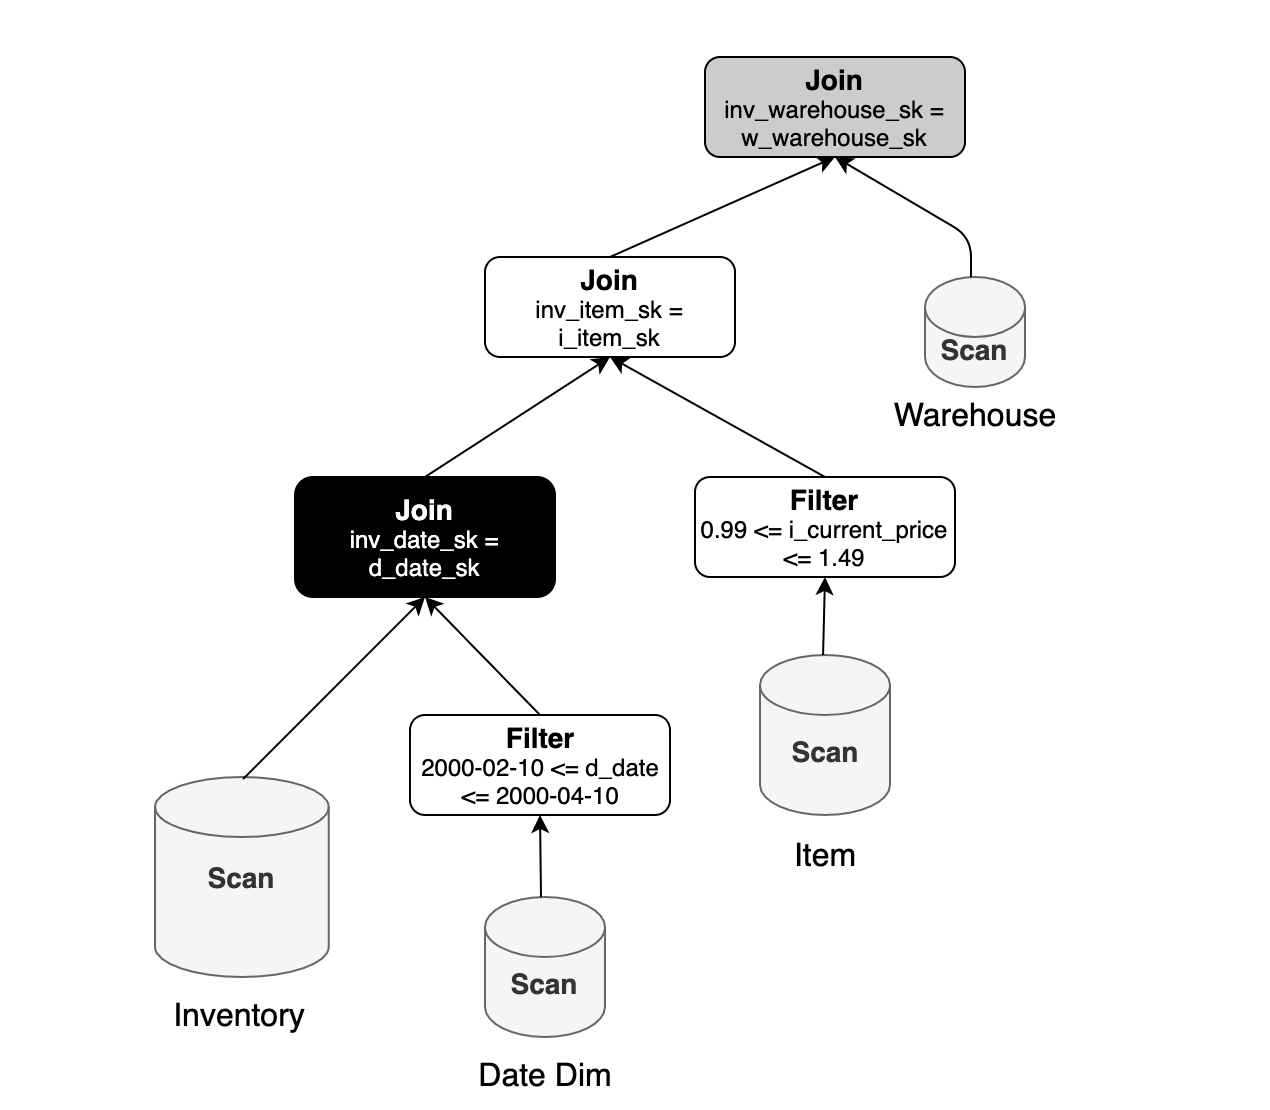
\includegraphics[width=7cm]{fig/with-reorder.png}}
\caption{Query 21 reordered}
\label{with-reorder}
\end{figure}